\chapter{Plasma spectrum}
\label{ch:spectrometry}
One of the fundamental characteristics of Plasma Coagulation Controller for medical applications is what species are produced and deposited during its application. Various studies observed the spectrum of plasma DBD discharge in air at atmosferic pressure and ambient temperature (\cite{DBDair_Trot}, \cite{DBDAirTypicalSpec}), it presents peaks relative to reactive species from water, oxygen, nitrogen and its oxides at visible wavelenght, from $\num{200}$ to $\SI{880}{\nano\meter}$.

We are intersted in plasma that contains molecules involved in blood coagulation mechanisms, Reactive Oxidant Species (such as hydroxil radical \ce{OH}) and Reactive Nitrogen Species (derived from nitric oxide \ce{NO}) (\cite{6153386}). In this spectroscopy study we give particular attention to them and their precursor, i.e. the presence of transitions relative to hydroxil, oxygen and molecular nitrogen.


\section{Optical Emission Spectroscopy}
The source produces plasma from a mixture gas of helium (or neon or argon) and air, along free electrons there are ions and species that collides with energetic electrons, and populate excited or metastable states with short lifetime. All reactive species partecipe in different reactions, and also in excitation and de-excitation reactions with conseguent emission of radiation. When an electron goes from state p at higher energy to state k of lower energy, is emitted radiation with central wavelenght $\lambda_0$. Power emitted by this radiation is given by radiant flux $d\phi_{\lambda}$ and selecting a solid angle as in figure, is possible to define radiance $L_{\lambda}$, and intensity $I$, as in equations \ref{eq:emission}. Intensity for a radiation ultimately depends on $n(p)$, population density for state p, and Einstein Coefficient for the transition $A_{pk}$ that is typical for the transition (\cite{book:291477}).

\begin{minipage}{.45\textwidth}
 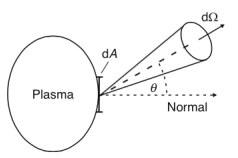
\includegraphics[width=0.8\textwidth]{Images/Spectroscopy/plasmaemission.png}
\end{minipage}
\begin{minipage}{.45\textwidth}
\begin{equation}
 \begin{split}
 &\lambda_{0} = \frac{hc}{E_p - E_k} \\
 &L_{\lambda} = \frac{d^2\phi_{\lambda}}{dA \cos(\theta) d\Omega} \\
 &I = \int L_{\lambda} d\lambda = n(p) A_{pk}
 \end{split} 
 \label{eq:emission}
\end{equation}
\end{minipage}

Using air as gas, composed by molecules, reaction that emits radiation in visible wavelenght are vibronic transitions where molecule goes from a vibrational state to another, with a change of vibrational quantum number $\nu$, and/or from a rotational state to another, with change of quantum number $J$ (\cite{book:137793}, \cite{wiki:vibronic}). When there is a vibrational transition, each line corresponds to different numbers $\nu'-\nu''$, these are transitions well spaced in the spectrum, easy to recognize. Rotational transitions gives birth to bands of peaks not space much, hard to resolve whitout an efficient spectrometer.

There are many reactions involving oxygen and nitrogen (see for example \cite{Kossyi_1992}), in this study we determine only principal transition observable with our spectrometer, to know dominant reactive species present in our plasma plume.

The experiments divides in emission line recognition and intensity measurements at different positions and with different gas mixtures.

\section{Line recognition}
We hypotize that plasma emission lines don't depend on which source we use, but on the discharge parameters, as described in chapter \ref{ch:electric}, we utilize prototype \textbf{A} presented before. A metal plate is positioned as target at a distance of $\SI{10}{\milli\meter}$ from plasma exit, as in figure \ref{fig:app1}. To start the dischare we use helium, with flow set to $\SI{2}{\liter/\minute}$.

For line recognition we utilize an IsoPlane spectrometer, that separates emissions with different wavelenghts with a grating. The spectrometer has a focal lenght of $\SI{320}{\milli\meter}$ and is equipped with three different gratings: $\num{150}$, $\num{1200}$ and \SI{2400}{gg/\milli\meter}, corresponding to different resolutions. %of $\num{0.26}$, $\num{0.03}$ and $\SI{0.01}{\nano\meter}$.
As in figure \ref{fig:app1}, light emitted by plasma is collected with a quartz lens %...
and passes trough an optical fiber %..
connected to the spectrometer entry, while at the spectrometer exit there is a CCD camera of $2048$ pixels and a count limit of $\num{65000}$.
\begin{figure}
\centering
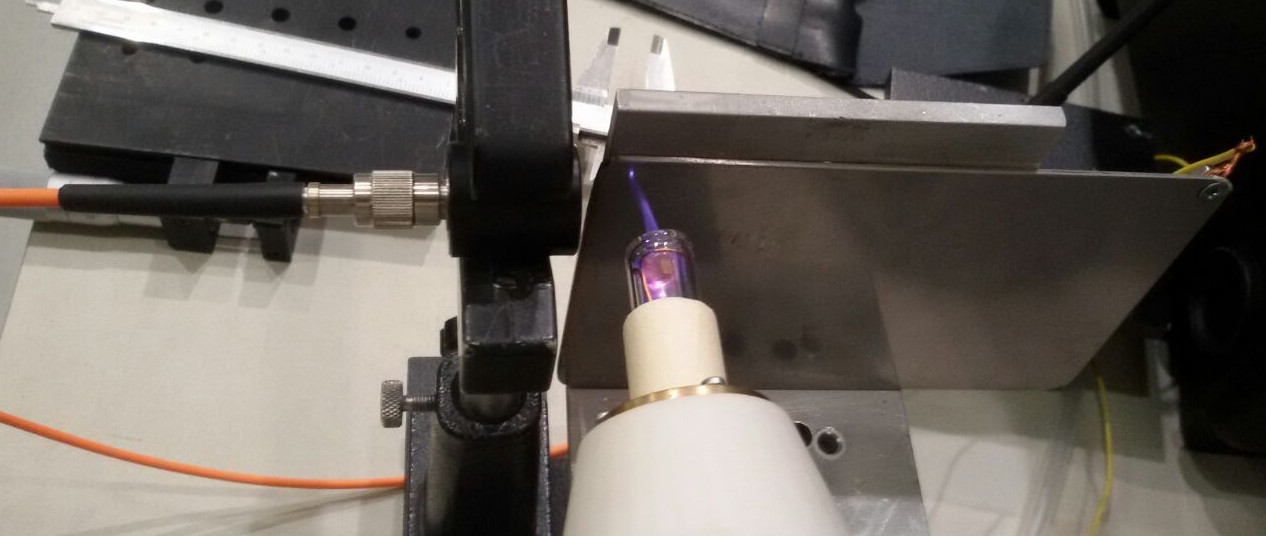
\includegraphics[width=.6\textwidth]{Images/Spectroscopy/apparato.jpg}
\caption{Setup of the experiment for line recognitizion: we can see the source, the metal target and the optical setup on the left. Plasma emission is collected by the lens and sent to the spectrometer.}
\label{fig:app1}
\end{figure}

Once a grating is chosen, we can set the start wavelenght on the acquisition system and from there it takes measures until the end of the CCD, for a specific wavelenght interval for every grating.
For each measure we select an appropriate acquisition time that allows to observe peaks with a good count number and avoid saturation.

It's important to stress out that, with this measuring method and due to complexity of plasma reactions and composition, it's not possible to extrapolate quantitative considerations between different species concentration. However it's possible to recognize the presence of certain species and make some considerations watching spectra variation with different experimental setup.


\subsection{Emission measurements}
To see what's generally produced in a discharge we take the spectrum for the entire wavelenght's region intersted, from $\num{230}$ to $\SI{800}{\nano\meter}$, with standard discharge paramters: $f \SI{5}{\kilo\hertz}$ and $\Delta t = \SI{15}{\micro\second}$.
First we do a rapid acquisition with the lowest resolution possible, to see intersting regions and have an idea of required exposition times. After that we do another acquisition with higher resolution for all wavelenghts, measuring several spectra. The entire spectrum is reconstructed attaching different spectra, showed in figure \ref{fig:spectr}, where are labelled principal transitions.
For every measure wa take also a background spectrum, without plasma, to recognize peaks that are not from the plasma.

We read data with IDL routines (\cite{GUMLEY200215}) and analyze it with ROOT \emph{TSpectrum.h} library (\cite{ROOT:TSpectrum}).
In every spectrum we divide each channel by the exposition time of the spectrum, evaluating the count rate at a specific wavelenght.
We estimate white noise contribution as the average value from a portion of the spectrum that doesn't presents peaks, and subtract it to count rates for each wavelenght.
In those spectrum we find emission peaks with TSpectrum functions (where is possible to set a treshold in heigth and the general width for lines to be searched) and isolate peaks from background. The exact wavelenght for each transition is found with a gaussian fit in an interval that takes into consideration the asymmetry where it's needed.

As said before, this study is focused on measure related to ROS and NRS, so in lines for \ce{NO}, \ce{OH} and \ce{N_2}.
\begin{figure}
\centering
\includegraphics[width=0.99\textwidth]{Images/Spectroscopy/spettrotot_unico_label_def.png}
\caption{Spectrum with an helium flow of $\SI{2}{\liter/\minute}$, pulse parameters of $f = \SI{5}{\kilo\hertz}$ and $\Delta t = \SI{16}{\micro\second}$. The emission is collected at the end of the nozzle, where plasma exits in air.}
\label{fig:spectr}
\end{figure}


\paragraph{\ce{NO} lines}
We observe two doublets for the transition $\ce{A^2\Sigma^+} \rightarrow \ce{X^2\Pi}$ with vibrational numbers (0-0) and (0-1) (\cite{Knie:166349}, \cite{VANSPRANG197955}), presented in table \ref{tab:spettroNO}. Intensities for the peaks are normalized with maximum value of $\num{1000}$ for the acquisition, the table shows as the intensities for this transition is very low. Other transition relative to this molecule have even lower relative intensity and are not observed in our study.
\begin{table}[h]
\centering
 \begin{tabular}{cc}
  \toprule
  $\lambda$ \text{[}\si{\nano\meter}\text{]} &\text{I [arb.u.]}\\
  \midrule
  \num{236.31(24)}  &27\\
  \num{237.00(15)}  &26\\
  \num{247.02(5)}  &28\\
  \num{247.86(12)}  &27\\
  \bottomrule
 \end{tabular}
 \caption{Peaks measured for \ce{NO}.}
 \label{tab:spettroNO}
\end{table}


\paragraph{\ce{OH} lines}
We find the rotational band for transition (\ce{A^2\Sigma}, $\nu' = 0$ $\rightarrow$ \ce{X^2\Pi}, $\nu'' = 0$), observing $13$ principal lines (\cite{doi:10.1142/S0129183100000857}).
In figure \ref{fig:OHsp} a zoom on the spectrum, in table \ref{tab:sptrOH} peak values.
\begin{figure}
 \centering
 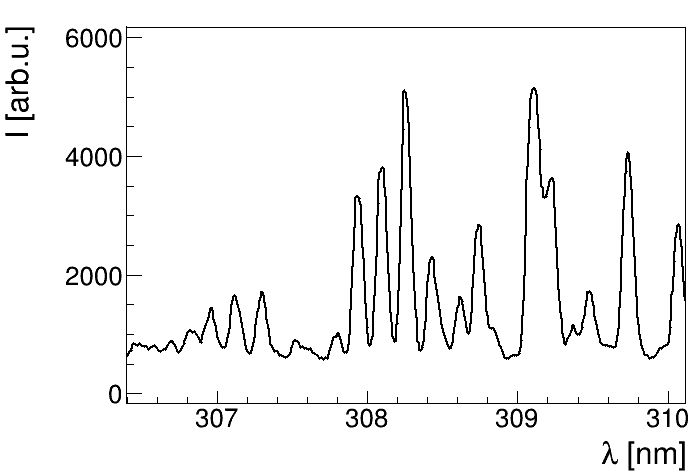
\includegraphics[width=0.6\textwidth]{Images/Spectroscopy/OH_f5t16v_2.png}
 \caption{Zoom on OH peaks}
 \label{fig:OHsp}
\end{figure}
\begin{table}
 \centering
 \begin{tabular}{cc}
  \toprule
  $\lambda$ \text{[}\si{\nano\meter}\text{]} &\text{I [arb.u.]}\\
  \midrule
  \num{306.96(1)}  &53\\
  \num{307.11(1)}  &58\\
  \num{307.29(1)}  &62\\
  \midrule                          
  \num{307.94(1)}  &142\\
  \num{308.09(1)}  &148\\
  \num{308.26(1)}  &161\\
  \num{308.43(1)}  &112\\
  \num{308.62(1)}  &46\\
  \num{308.74(1)}  &137\\
  \midrule                          
  \num{309.11(1)}  &151\\
  \num{309.22(1)}  &120\\
  \num{309.45(1)}  &36\\
  \num{309.73(1)}  &125\\
  \bottomrule
 \end{tabular}
 \caption{Peaks measured for \ce{OH}.}
 \label{tab:sptrOH}
\end{table}


\paragraph{\ce{N_2} and \ce{N+_2} lines}
Measured spectrum presents several lines relative to nitrogen molecules, including the strongest, for diatomic molecule dinitrogen. We observe the Second Positive System for \ce{N2} transition $\ce{C^3\Pi} \rightarrow \ce{B^3\Pi}$ and the First Negative System for \ce{N2+} transition $\ce{B^2\Sigma} \rightarrow \ce{X^2\Sigma}$, in table \ref{tab:sptrN} peak values (\cite{N2lab}, \cite{Britun_2007}). For \ce{N2} is found also a band of multiple rotational lines centered around \SI{336.58(1)}{\nano\meter}.
Some of the peaks are seen in the second diffraction order, where there is more distance between lines. In figure \ref{fig:N2} we presente two zooms for \ce{N2} lines.
\begin{figure}
 \centering
 \subfloat[Transitions with $\Delta \nu = 2$]{
    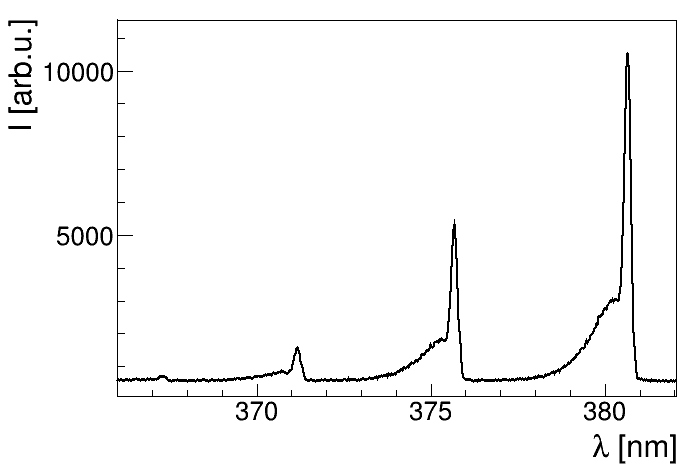
\includegraphics[width=0.45\textwidth]{Images/Spectroscopy/N2v_f5t16_2.png}
 }
 \hfill
 \subfloat[Strongest line (0-0), $2^{\text{nd}}$ diffraction order]{
    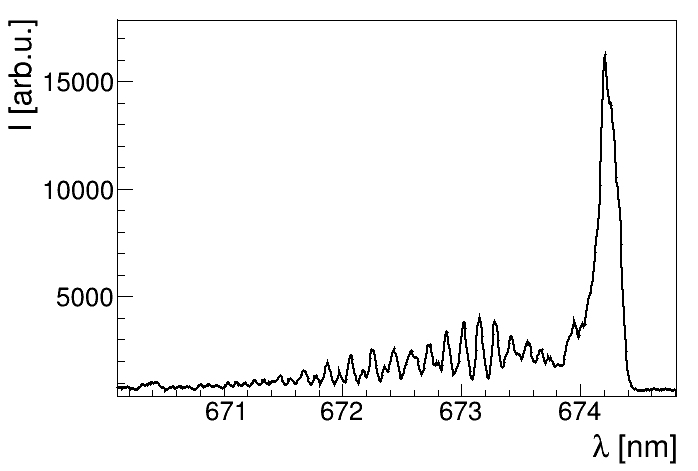
\includegraphics[width=0.45\textwidth]{Images/Spectroscopy/N2r_f5t16_2.png}
 }
 \caption{Zoom on \ce{N2} transitions.}
 \label{fig:N2}
\end{figure}

\begin{table}
\centering
 \begin{tabular}{cccc}
  \toprule
                            &$\lambda$ \text{[}\si{\nano\meter}\text{]} &\text{I [arb.u.]}  &($\nu'-\nu''$)\\
  \midrule
  \multirow{3}*{\ce{N_2}}   &\num{316.03(1)}  &381  &(1-0)\\
                            &\num{337.11(1)}  &1000 &(0-0)\\
                            &\num{357.77(1)}  &722  &(0-1)\\
  \midrule
  \multirow{4}*{\ce{N_2}}   &\num{367.22(20)}  &58  &(3-5)\\
                            &\num{371.12(4)}  &172  &(2-4)\\
                            &\num{375.66(2)}  &232  &(1-3)\\
                            &\num{380.64(2)}  &423  &(0-2)\\
  \midrule
  \multirow{2}*{\ce{N_2^+}} &\num{391.50(2)}  &355  &(0-0)\\
                            &\num{427.45(2)}  &180  &(0-1)\\
  \bottomrule
 \end{tabular}
 \caption{Peaks measured for \ce{N_2} and \ce{N+_2}.}
 \label{tab:sptrN}
\end{table}


\paragraph{Atomic lines}
We observe other lines from elements present in the plume (\cite{NIST}):
\begin{itemize}
 \item \textbf{\ce{H_{\alpha}}} line corresponding to transition from quantum number $n=3$ to $n=2$
 \item \textbf{\ce{He}} two of the strongest lines for helium
 \item \textbf{\ce{O}} strong line of oxygen
\end{itemize}
\begin{table}
\centering
 \begin{tabular}{ccc}
  \toprule
                            &$\lambda$ \text{[}\si{\nano\meter}\text{]} &\text{I [arb.u.]}\\
  \midrule
  \ce{H_{\alpha}}           &\num{655.96(4)}  &113\\
  \midrule
  \multirow{2}*{\ce{He}}    &\num{586.94(5)}  &122\\
                            &\num{705.56(1)}  &649\\
  \midrule
  \ce{O}                    &\num{776.89(1)}  &393\\
  \bottomrule
 \end{tabular}
 \caption{Lines measured for \ce{H}, \ce{He} and \ce{O}.}
 \label{tab:sptrother}
\end{table}


\section{Relative intensities}
To understand the mechanisms of plasma expulsion and deposition, we measure plasma emission intensity varying voltage peak values, line of sight of the spectrometer and gas composition.

\subsection{Pulse settings}
We measure emission lines with different parameters for the voltage pulse, utilizing the same experimental apparatus as before. As seen in chapter \ref{ch:electric} for different pulse repetition rates we have the same electric behavior, but this parameter could still influence species production rates.

%Reactions that produce and recombine reactive species, and consequently density and lifetime of species, are influenced by electric field and duration of the discharge.
We observe spectra with three different parameter combinations, corresponding to different intensity of the treatment:
\begin{itemize}
 \item low: $f = \SI{5}{\kilo\hertz}$ and $\Delta t = \SI{15}{\micro\second}$
 \item medium: $f = \SI{10}{\kilo\hertz}$ and $\Delta t = \SI{10}{\micro\second}$
 \item high : $f = \SI{15}{\kilo\hertz}$ and $\Delta t = \SI{10}{\micro\second}$
\end{itemize}

For every setting we collect plasma emission along two different line of sight:
\begin{itemize}
 \item position 1: as close as possible to the end of the nozzle, near plasma exit point from the source;
 \item position 2: close to the target, at \SI{10}{\milli\meter} from plasma exit point, where it collides with target.
\end{itemize}

We evaluate intensities for \ce{OH} and \ce{N2} species, collectively for the lines in a wavelength range specific for the peaks. For \ce{OH} lines is considered all the rotational band between $\num{306}$-\SI{309}{\nano\meter}, lines for \ce{N2} are separated in those between $\num{335}$-\SI{337}{\nano\meter} (rotational band and (0-0) transition) and those between $\num{368}$-\SI{382}{\nano\meter} (vibrational transitions with $\Delta \nu = 2$).

In figure \ref{fig:irel} we present measurements result for considered lines. .

Intensities for \ce{OH} decreases drastically increasing the distance from the source, in position 2 we find values lower than $0.1\%$ of those from position 1. \ce{OH} lines for both positions have same intensity with low and medium power setup, while is lower with higher frequency, with similar behavior in both positions.

Also \ce{N2} intensities depend on pulse repetition rate: they decrease with higher pulse rates, for every lines, reaching around $0.6\%$ for $f = \SI{15}{\kilo\hertz}$ in position 1, and lower values for position 2.

It seems that production of both those reactive species have rates dependant from pulse repetition rates, in particular the intensity of their emission decreases at higher frequencies.
\begin{figure}
\centering
 \subfloat[\ce{OH} intensities in range $\num{306}$-\SI{309}{\nano\meter}]{
    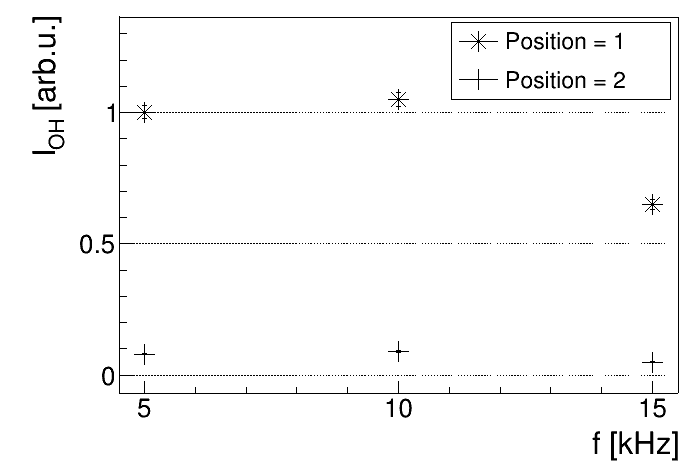
\includegraphics[width=0.48\textwidth]{Images/Spectroscopy/If_OH.png}
 }
 \hspace{0.55\textwidth}
 \subfloat[\ce{N2} intensities range $\num{335}$-\SI{337}{\nano\meter}]{
    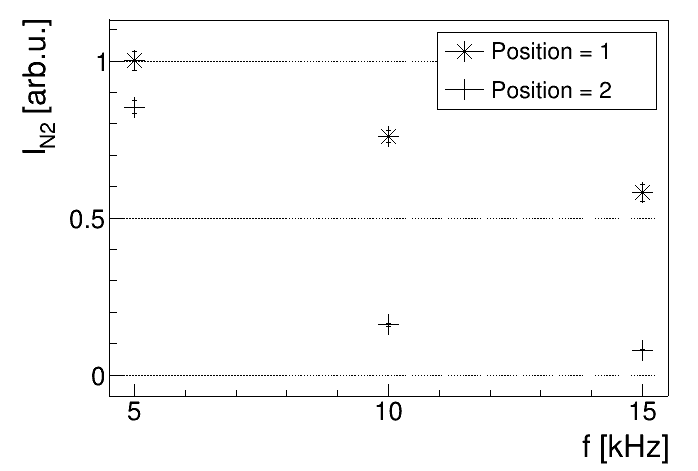
\includegraphics[width=0.48\textwidth]{Images/Spectroscopy/If_N2r.png}
 }
 \hfill
 \subfloat[\ce{N2} intensities range $\num{368}$-\SI{382}{\nano\meter}]{
    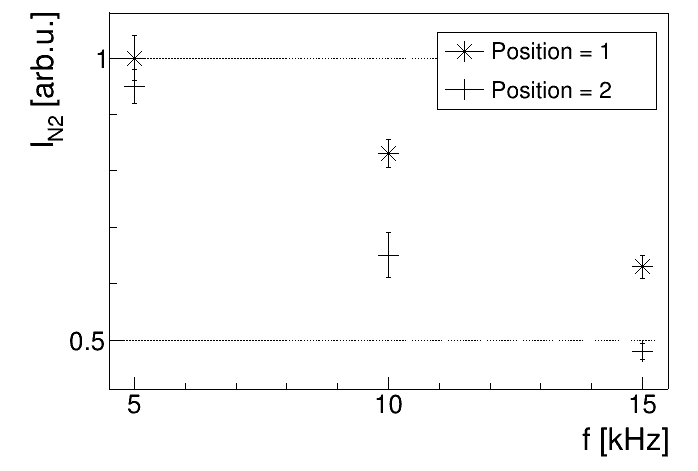
\includegraphics[width=0.48\textwidth]{Images/Spectroscopy/If_N2v.png}
 }
 \caption{Relative intensities of selected portions of the spectrum, for different pulse repetition rates, for position 1 and position 2.}
 \label{fig:irel}
\end{figure}


\subsection{Position}
We want to analyze plasma emission at different positions with the other source analyzed in this work, prototype \textbf{B} in chapter \ref{ch:electric}, in a similar way to what we did in the previous measurements. The setup is similar to the one described in chapter \ref{ch:shape}: as in figure \ref{fig:app2}, we utilize the glass nozzle and a conductive target at \SI{10}{\milli\meter} from its end.
\begin{figure}
\centering
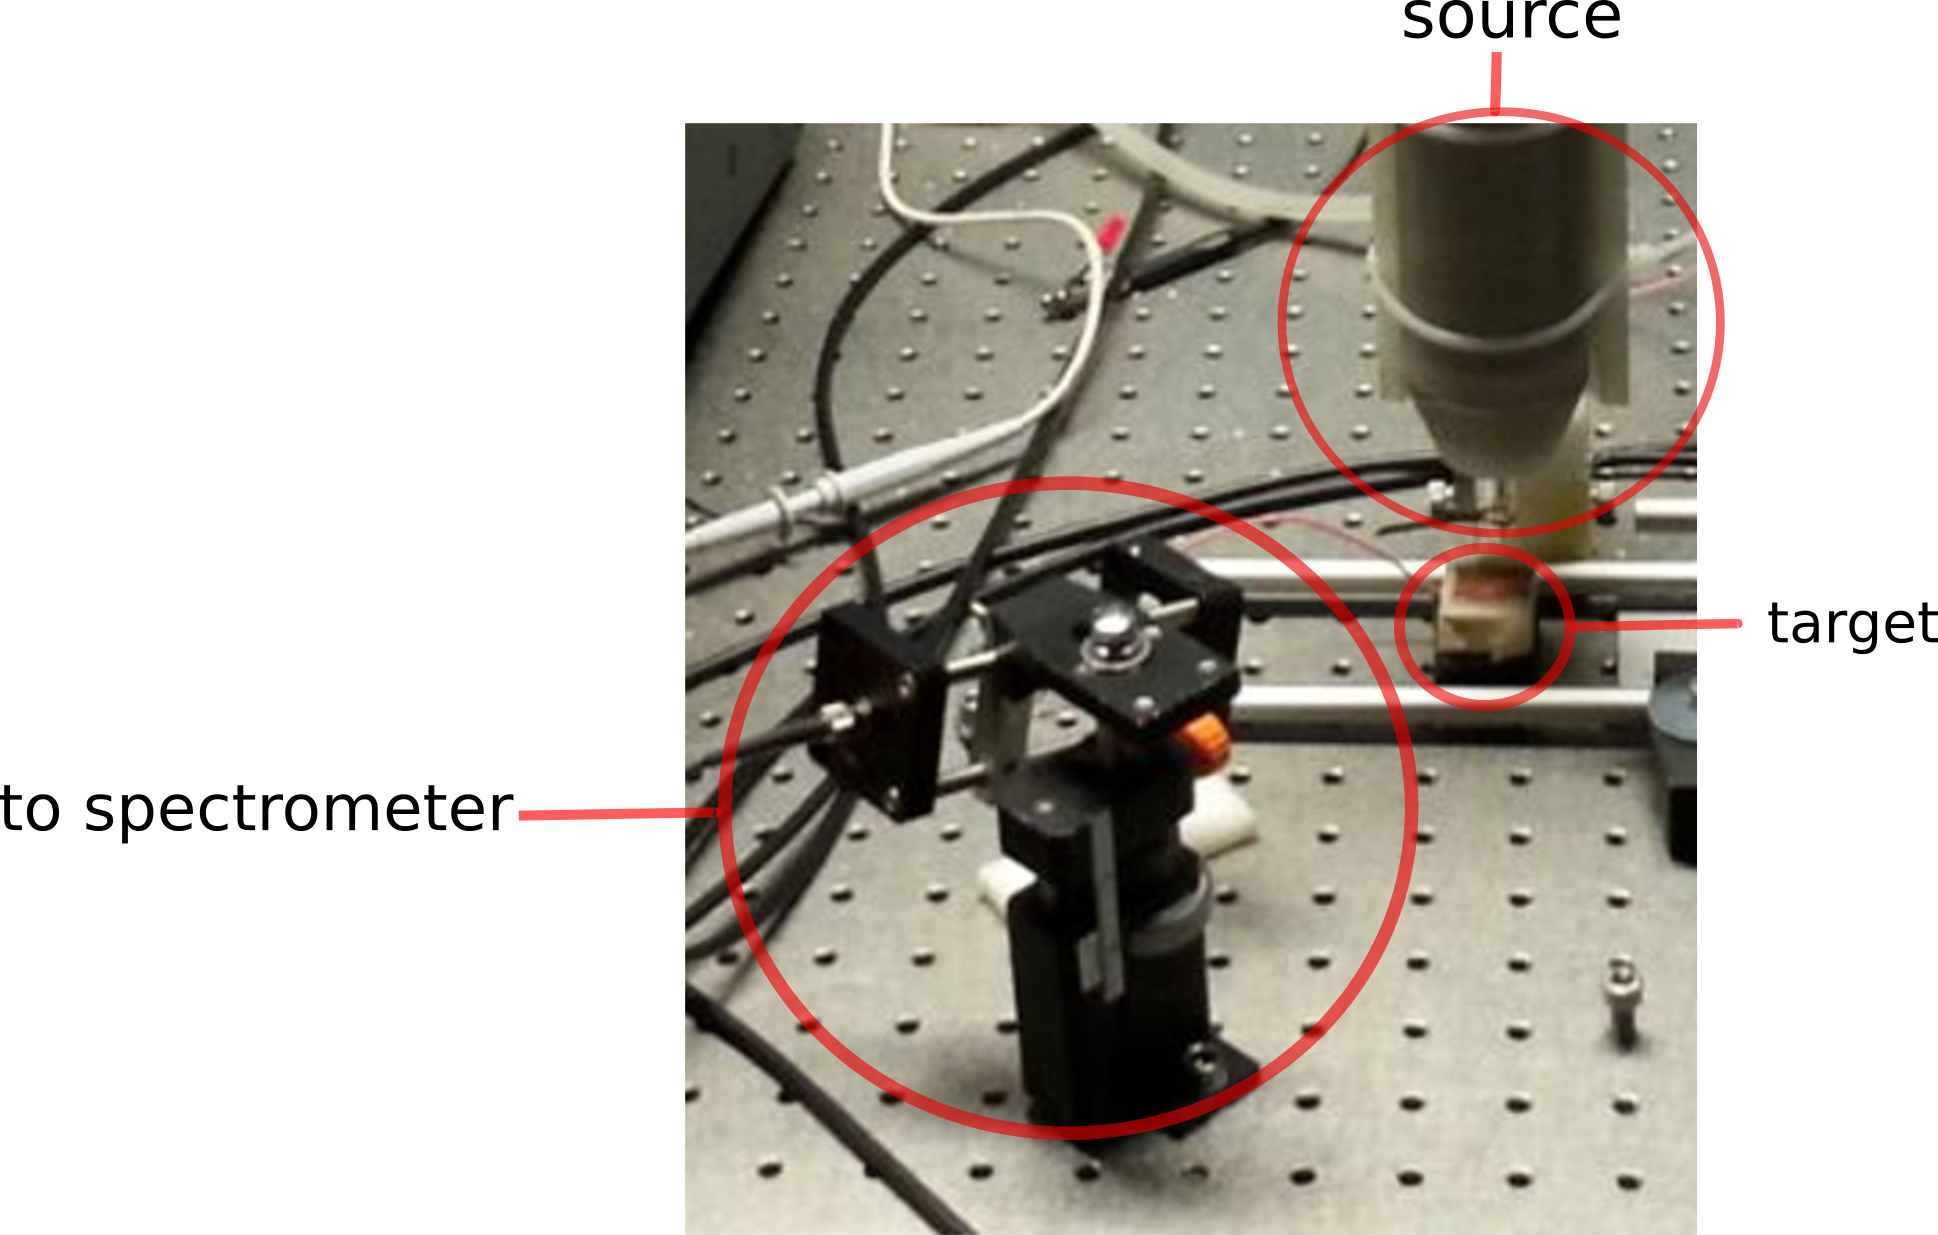
\includegraphics[width=.7\textwidth]{Images/Spectroscopy/app2_lines.png}
\caption{Setup of the esperiment for intensity measurements: we can see spectrometer's lens on the left, the source and the metal target.}
\label{fig:app2}
\end{figure}

We utilize a mini-spectrometer \emph{Hamamatsu C10082CAH}, with resolution of \SI{1}{\nano\meter}, spectral range from \SI{200}{\nano\meter} to \SI{800}{\nano\meter} and a CCD sensor \emph{S10420-1106} with \num{2048} pixels. We find the efficiency of the spectrometer for different wavelenghts with measurements of emission from a lamp with known emission spectrum.

To produce plasma we use three different gasses: helium with a flow of \SI{2}{\liter/\minute}, neon with gas flow \SI{2.5}{\liter/\minute} and argon with flow \SI{2}{\liter/\minute}.

The experimental setup allows to measure plasma emission at different heights along the nozzle axis, we evaluate intensity in four different positions:
\begin{itemize}
 \item \SI{-5}{\milli\meter}, inside the nozzle
 \item \SI{0}{\milli\meter}, at the end of the nozzle
 \item \SI{5}{\milli\meter}, between nozzle and target
 \item \SI{10}{\milli\meter}, right before target position
\end{itemize}

We consider the total emission for the entire spectral range \num{200}-\SI{800}{\nano\meter} and the relative emission for some selected lines, different for the different gasses:
\begin{itemize}
 %\item UVB lines : doublet centered at \SI{293.2}{\nano\meter} and \SI{295.5}{\nano\meter} that could be emitted by \ce{NO} molecules, but we can not be sure due to spectrometer's low resolution;
 \item \ce{N_2} : three lines centered at \SI{364.2}{\nano\meter} (transition $(1-0)$), \SI{383.0}{\nano\meter} (transition $(0-0)$) and \SI{403.9}{\nano\meter} (transition $(2-4)$);
 \item \ce{He} : one line at \SI{446.2}{\nano\meter};
 \item \ce{Ne} : one doublet at \SI{628.8}{\nano\meter} and \SI{630.6}{\nano\meter}, one doublet at \SI{639.2}{\nano\meter} and \SI{641.0}{\nano\meter} and a single line at \SI{683.1}{\nano\meter};
 \item \ce{Ar} : three different lines at \SI{722.9}{\nano\meter}, \SI{734.0}{\nano\meter} and \SI{772.6}{\nano\meter}.
\end{itemize}


Results are in figure \ref{fig:Irel_pos}. We normalize total intensities to compare emissivity variation for different positions, while relative intensities are divided for the respective total intensity and multiplied for spectrometer efficiency for considered wavelenght.
When we use helium to start plasma, emission is lower inside the nozzle, increase at the exit and decreases slightly moving towards the target. For other gasses emission decreases increasing distance from the source.
For every gas, emission from \ce{N_2} increases until it reaches a constant value.
Lines from specific gasses decreases distant from the nozzle, with slope different for different gasses.
It's intersting to note how neon emission decreases linearly, while \ce{N_2} emission increases and it's an effect that we can see visually: going from the nozzle to the target plasma color goes to red (neon emission) to violet (nitrogen emission).
\begin{figure}
\centering
  \subfloat[Total emission intensity.]{
    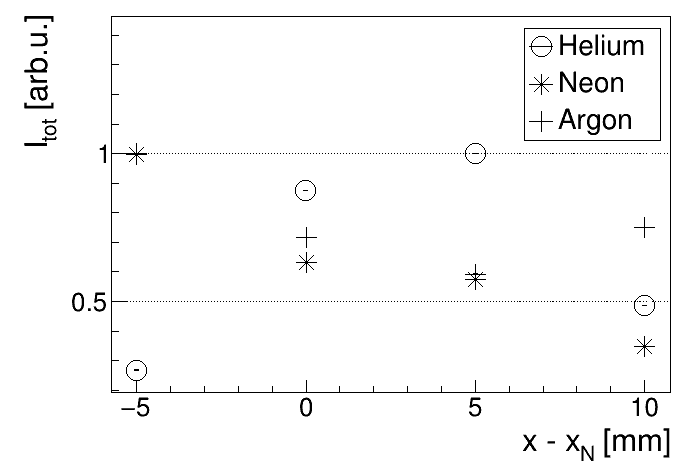
\includegraphics[width=0.48\textwidth]{Images/Spectroscopy/Itot_pos2.png}
  }
  
  %\subfloat[UVB lines]{
  %  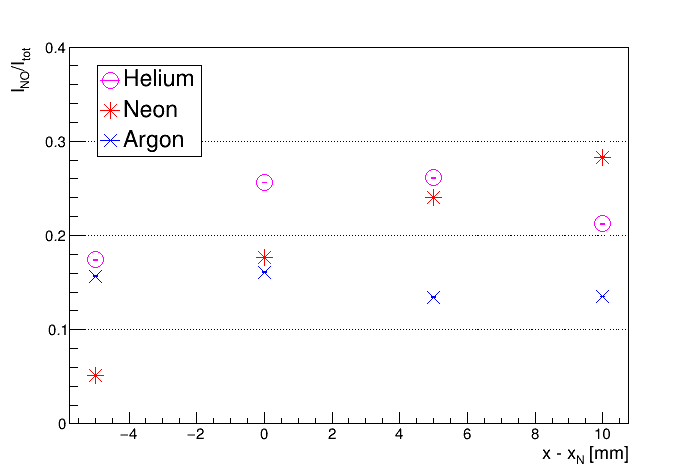
\includegraphics[width=0.48\textwidth]{Images/Spectroscopy/Irel_NO_pos.png}
  %}
  
  \subfloat[\ce{N_2} lines]{
    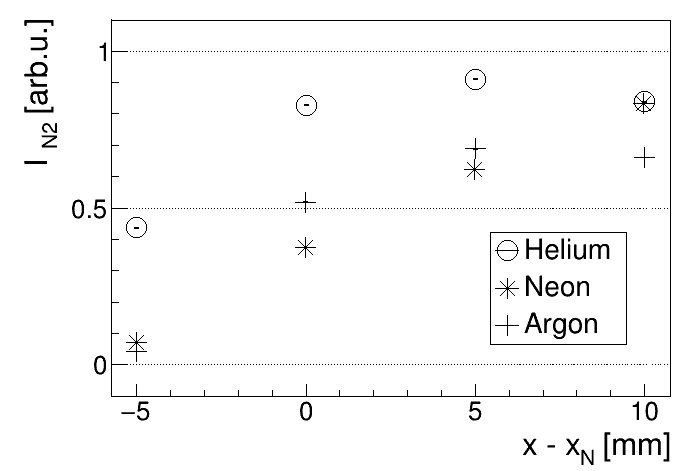
\includegraphics[width=0.48\textwidth]{Images/Spectroscopy/Irel_N2_pos2.png}
  }
  \hfill
  \subfloat[\ce{He} lines, \ce{Ne} lines, \ce{Ar} lines.]{
    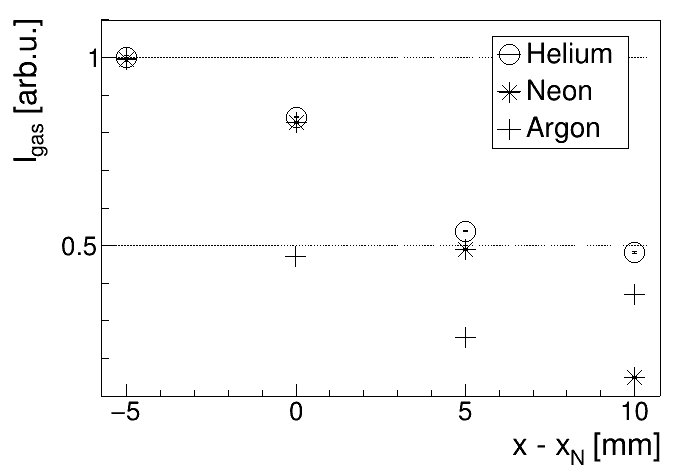
\includegraphics[width=0.48\textwidth]{Images/Spectroscopy/Irel_gas_pos2.png}
  }
\caption{Behavior of total intensities (a) and relative intensities for selected portions of the spectrum (b-c-d), changing spectrometer's line of sight, with different starting gas. At \SI{0}{\milli\meter} the lens points at the end of the nozzle, at \SI{10}{\milli\meter} at a metal target. Relative intensities in (d) are for lines corresponding to the element that we use as starting gas. Relative intensities take into consideration spectrometer's efficiency and total emission for every position.}
 \label{fig:Irel_pos}
\end{figure}

As we could expect we see that inside the nozzle the emission depends from the gas we use to start the plasma, going outside emission due to nitrogen species becames dominant in the discharge.

\subsection{Gas composition}
We use helium as starting gas, mixed with argon or nitrogen using specific flowmeters, that allows to add up to \SI{0.2}{\liter/\minute}, with resolution of \SI{0.01}{\liter/\minute}.
If we set the helium flow to \SI{2}{\liter/\minute}, we can have gas mixtures where argon and nitrogen have a maximum percentage of $\num{10}\%$.

We point the spectrometer at the end of the nozzle and collect spectra for three different gas concentrations, finding the intensities in figure \ref{fig:Irel_flow}.
When we add nitrogen to the gas, total emission intensity lowers, while nitrogen emission doesn't change as expected. We have this result because we are increasing very slightly nitrogen concentration respect to the quantity naturally present in air, it means that at the end of the nozzle we alredy see all possible nitrogen emission due to molecules naturally present in air.
When we add argon, the total emission increases, while relative emission from elements other than argon decreases slightly, as we expect if we add he argon lines to the total sum. It means that the only variation when we add argon is that we see the emission relative to this element, the emission relative to other elements stays unchanged.
\begin{figure}
\centering
  \subfloat[Total emission intensity.]{
    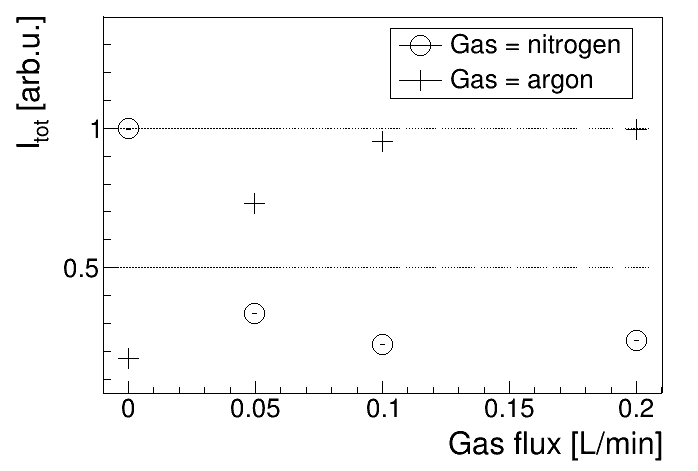
\includegraphics[width=0.48\textwidth]{Images/Spectroscopy/Itot_flux2.png}
  }
  
  %\subfloat[UVB lines]{
  %  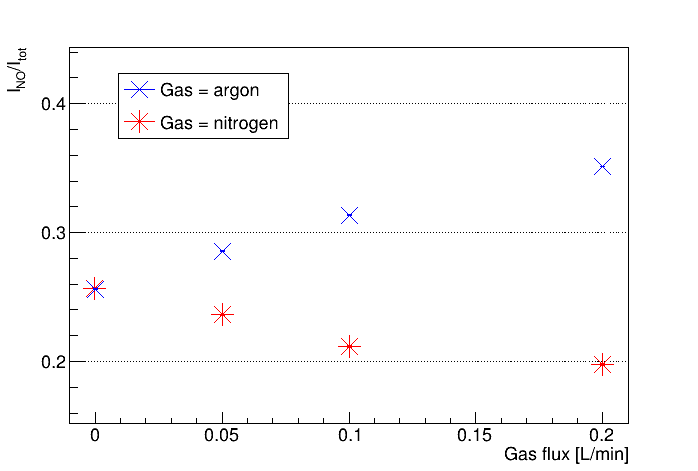
\includegraphics[width=0.48\textwidth]{Images/Spectroscopy/Irel_NO_flux.png}
  %}
  
  \subfloat[\ce{N_2} lines]{
    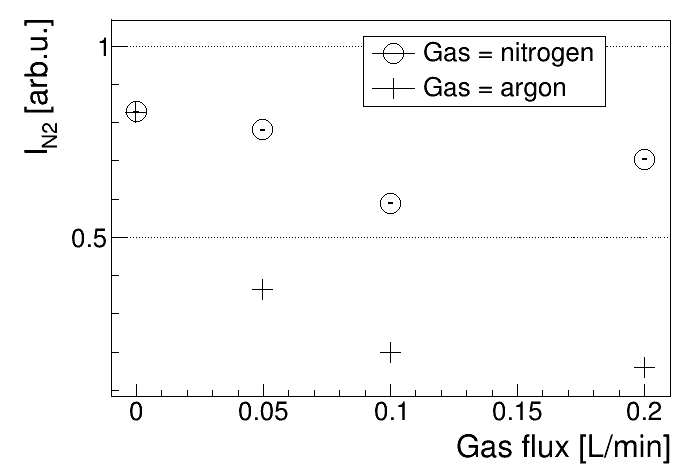
\includegraphics[width=0.48\textwidth]{Images/Spectroscopy/Irel_N2_flux2.png}
  }
  \hfill
  \subfloat[\ce{He} line]{
    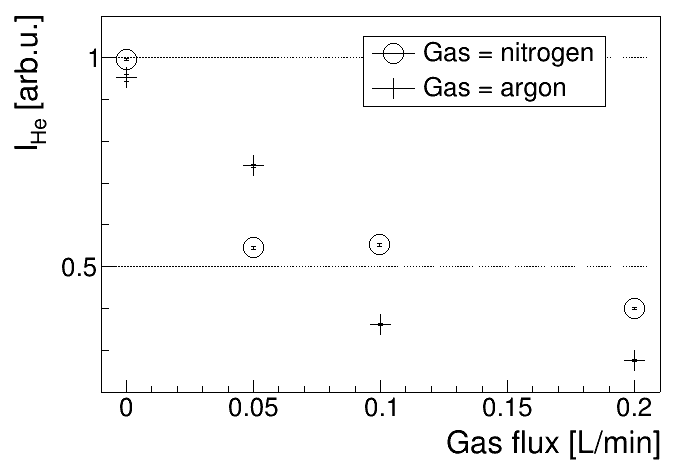
\includegraphics[width=0.48\textwidth]{Images/Spectroscopy/Irel_He_flux2.png}
  }
  
  \subfloat[\ce{Ar} line for argon gas mixture]{
    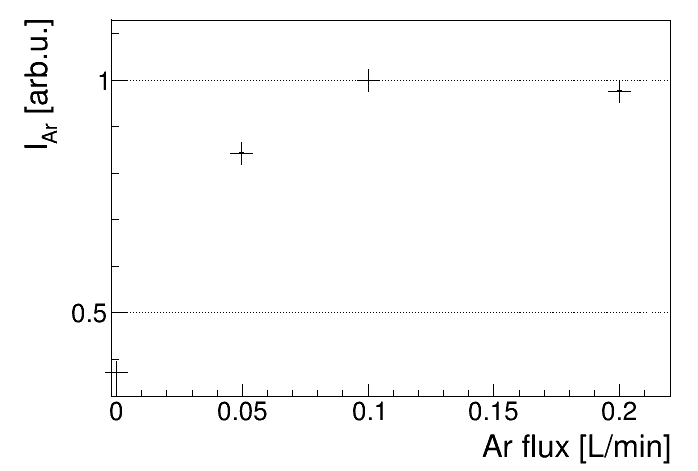
\includegraphics[width=0.48\textwidth]{Images/Spectroscopy/Irel_Ar_flux2.png}
  }
\caption{Behavior of total intensities (a) and relative intensities for selected portions of the spectrum (b-c-d-e), changing the composition of the gas. A flow of \SI{0.2}{\liter/\minute} corresponds to the $\num{10}\%$ of the total gas flow. Relative intensities take into consideration spectrometer's efficiency and total emission for every gas mixture.}
 \label{fig:Irel_flow}
\end{figure}


\section{Estimation of plasma temperatures}
From diatomic molecule's spectra it's possible to evaluate some parameters that are indicators of plasma's state: rotational temperatures for \ce{OH} and \ce{N2}, $T_{r}$, and vibrational temperature for \ce{N2}, $T_{v}$.
These parameters are estimation of the temperature at which thermal energy is comparable to the gap energy between rotational or vibrational state transitions, they can be defined as in equations \ref{eq:temperatures} where $\nu$ is the vibrational quantum number and $I$ is the quantizied moment of inertia of the molecule.
\begin{equation}
 \centering
 \begin{split}
  &T_{r} = \frac{\hslash^2}{2 k_{B} I}\\
  &T_{v} = \frac{h \nu}{k_{B}}
 \end{split}
 \label{eq:temperatures}
\end{equation}

Rotational temperatures can be considered an estimation of neutral gas kinetic temperature. Vibrational temperature gives an idea of the population of vibrational states, useful to determine chemical reactions inside plasma.

\subsection{Rotational temperature for \ce{OH} and for \ce{N2}}
In rotational bands the intensity of a transition for a specific wavelength is proportional to the number density popolation of upper state (equation \ref{eq:emission}), that, considering a Maxwell-Boltzmann distribution, is proportional to the temperature of the species. In equation \ref{eq:Irot} the proportionality is explicitated, with $D_{0}$ parameter that depends on number of initial molecules, partition function of the rotational state and quantum rotational numbers for upper and lower state, $S$ is the oscillator strenght specific for the molecule and $E_{r}$ depends from a constant defined by the vibrational state and from quantum rotational number for upper state (\cite{MOON2003249}).
\begin{equation}
 \centering
 I = \left(\frac{2 \pi}{\lambda}\right)^4 D_0 S \exp\left(-\frac{E_r}{k_B T_r}\right)
 \label{eq:Irot}
\end{equation}

As explained before, rotational bands have many lines, not distinguishable with our spectrometer, an approach to temperature estimation is to simulate spectra with different temperatures and to minimize differences for measured spectrum (\cite{Izarra_2000}).
In a predetermined range of temperatures we simulate different spectra with different temperatures, where each line is a gaussian peak with its width that takes into consideration broadning due to thermal motion, Doppler effect and measure resolution. For every spectrum we estimate the mean square difference and select the temperature associated with the minimum differance, while we estimate the error taking an upper and a lower limit where difference is larger by $5\%$ of the minimum value. An example of the spectra is in figure \ref{fig:Trfit}, while resulting temperatures are in figure \ref{fig:Trval}.
\begin{figure}
\centering
  \subfloat[\ce{OH}]{
    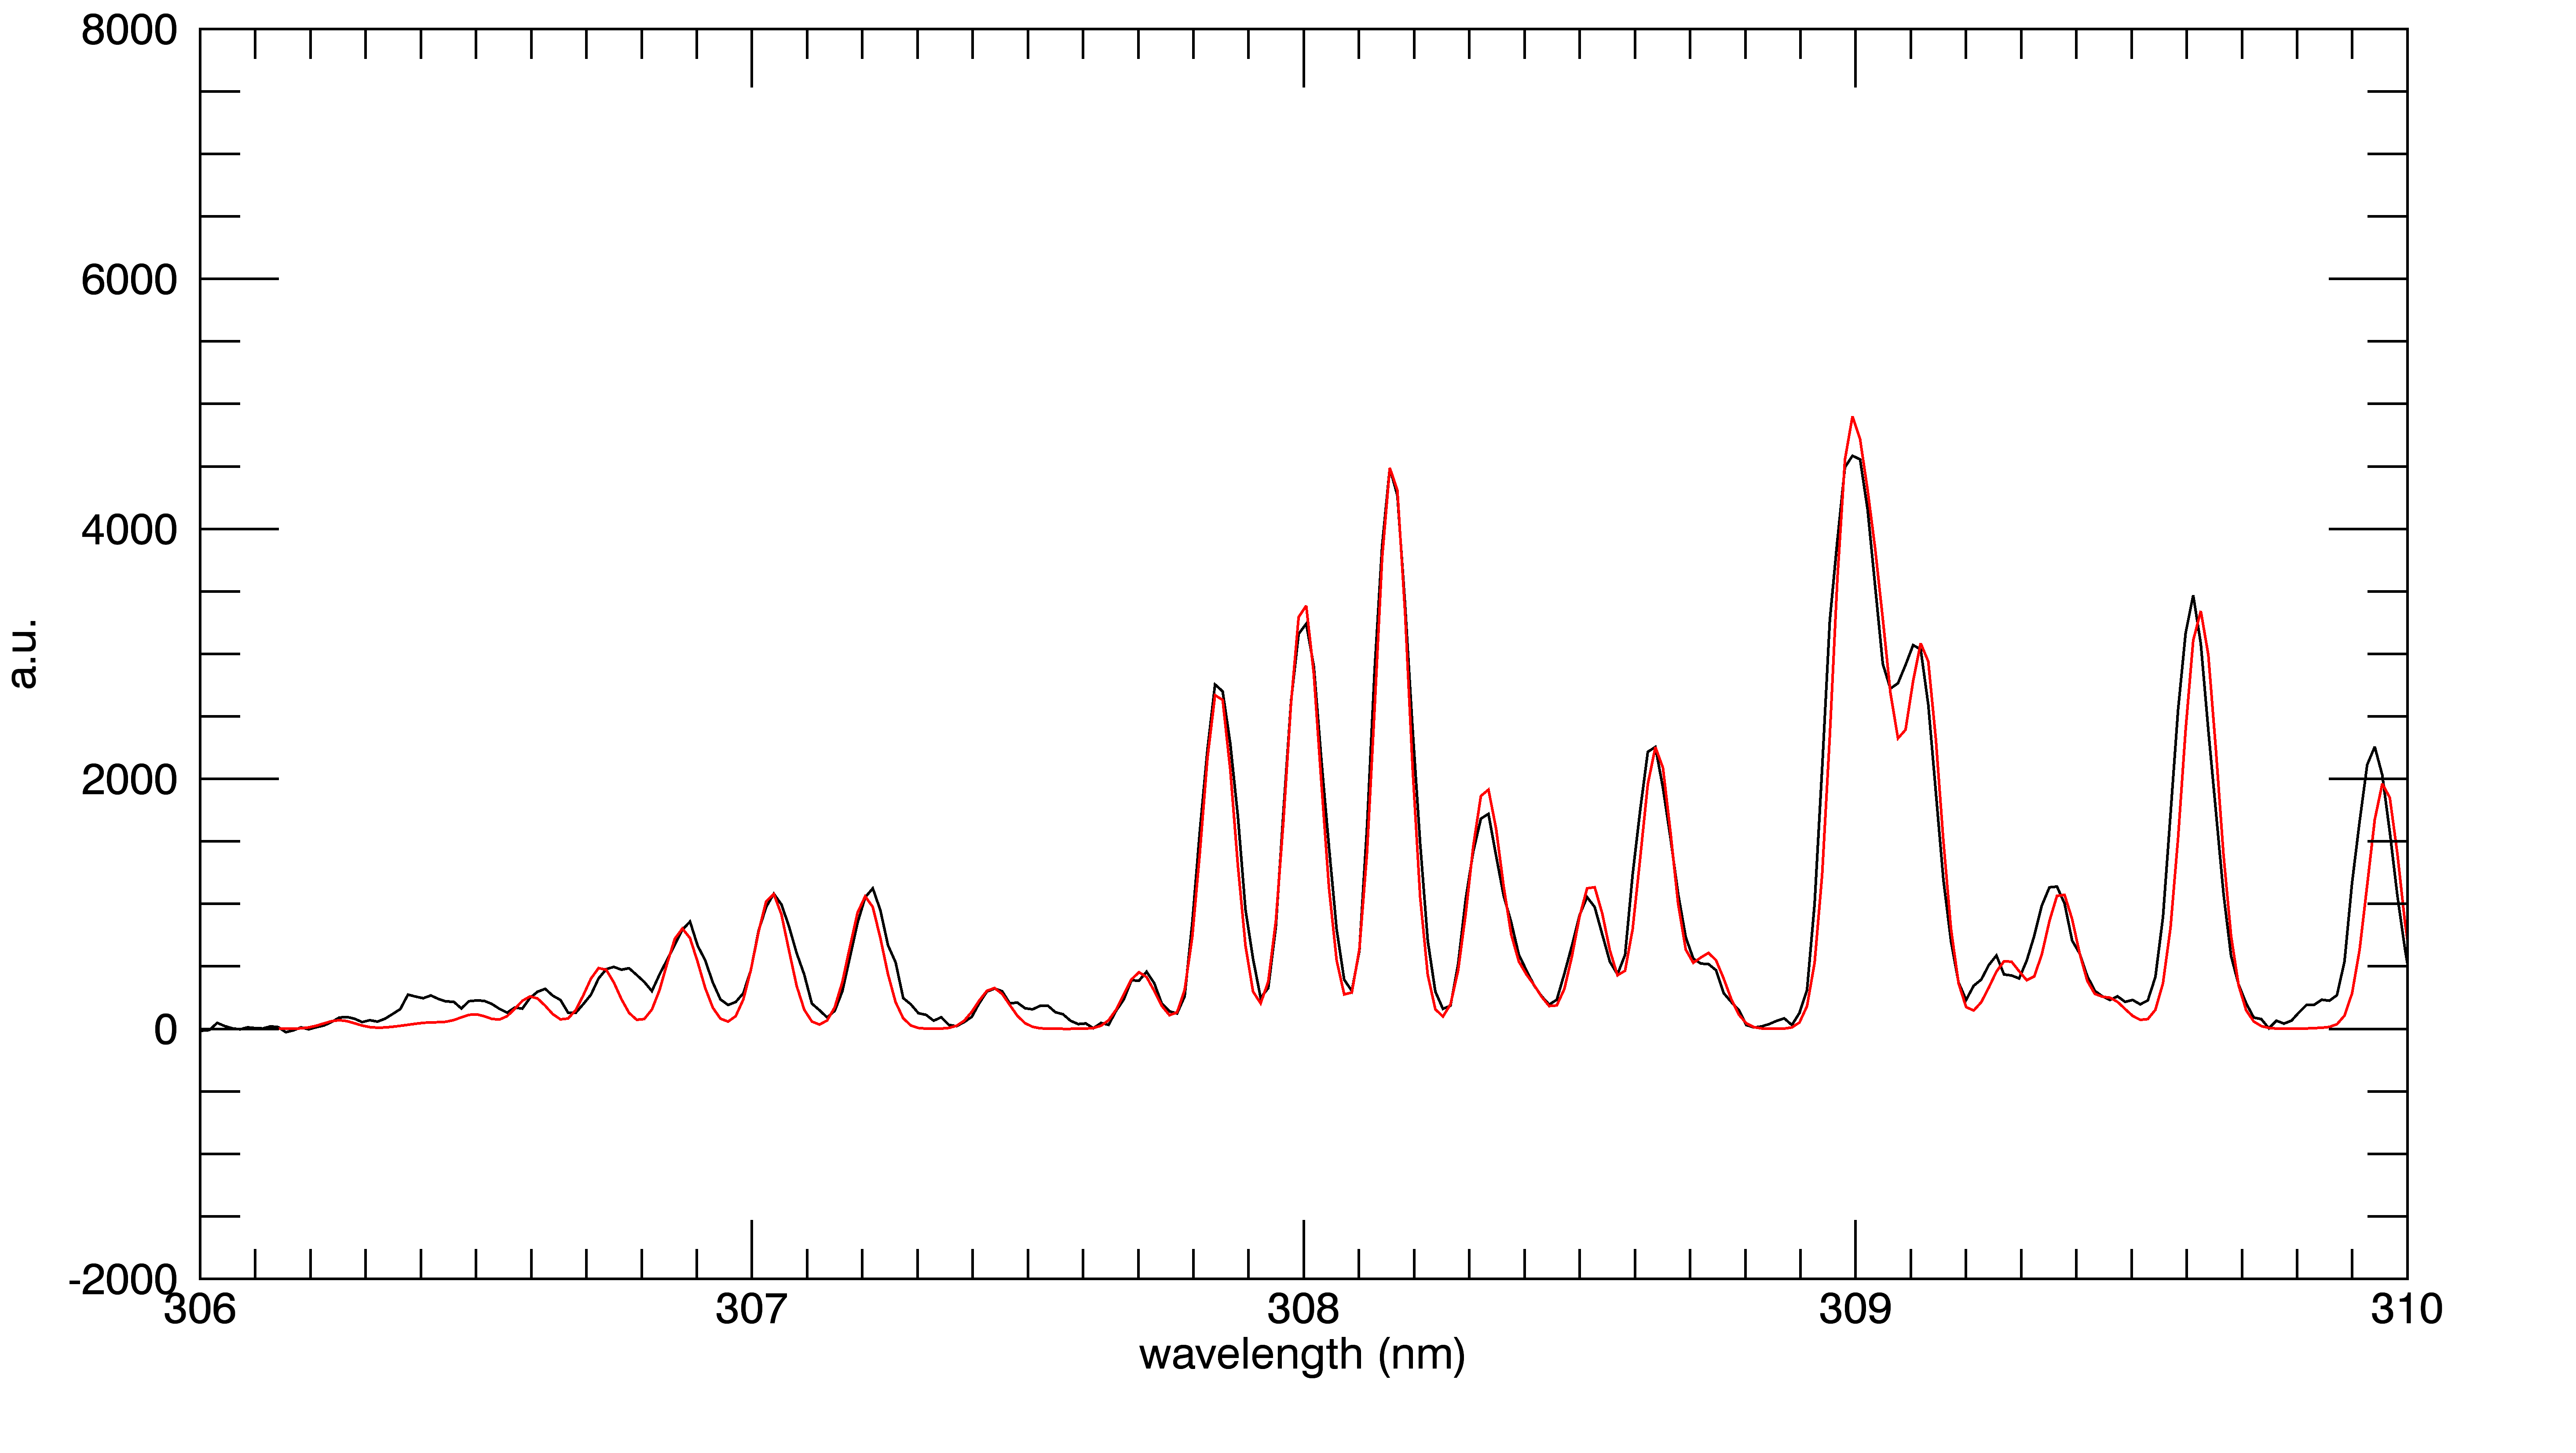
\includegraphics[width=0.48\textwidth]{Images/Spectroscopy/OHFit_f5t16elio.png}
  }
  \hfill
  \subfloat[\ce{N_2}]{
    \includegraphics[width=0.48\textwidth]{Images/Spectroscopy/N2rotFit_elio.png}
  }
 \caption{Example of optimal spectrum simulation for \ce{OH} and \ce{N_2} considered species.}
 \label{fig:Trfit}
\end{figure}


From estimated temperatures we can see that they are compatible with each other, for every distance and for every pulse setup. It's then possible to evaluate a mean value for the species, that are $T_{r,\ce{OH}} = \SI{352(38)}{\kelvin}$ and $T_{r,\ce{N2}} = \SI{321(41)}{\kelvin}$, compatible with each other, and that, as said before, can be taken as an indicator of kinetic temperature for neutral species, so as temperature of the fluid. Those temperatures are a little higher then room temperature, but they are compatible with the definition of cold plasma.
\begin{figure}
\centering
  \subfloat[\ce{OH}]{
    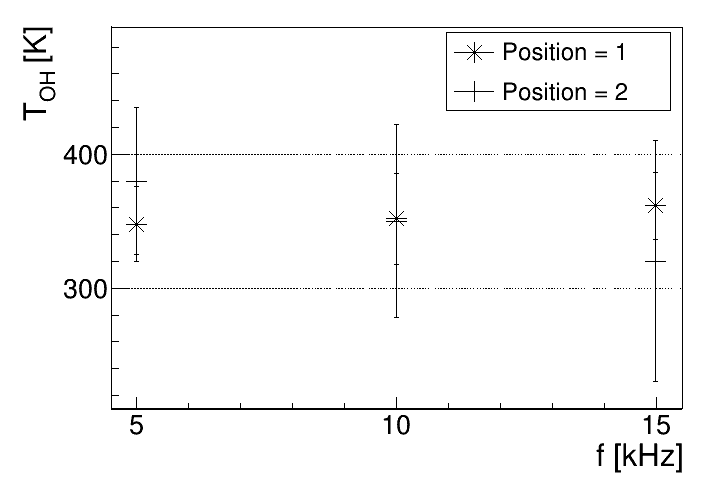
\includegraphics[width=0.48\textwidth]{Images/Spectroscopy/TrOH2.png}
  }
  \hfill
  \subfloat[\ce{N2}]{
    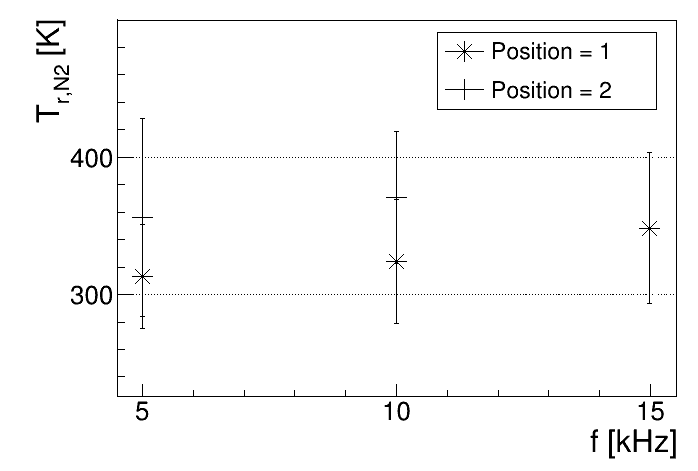
\includegraphics[width=0.48\textwidth]{Images/Spectroscopy/TrN2_2.png}
  }
 \caption{Estimation of rotational temperature of \ce{OH} and \ce{N2} molecules, for different parameters setup and positions.}
 \label{fig:Trval}
\end{figure}

\subsection{Vibrational temperature for \ce{N_2}}
Given a set of vibrational transition lines with defined $\Delta \nu = \nu' - \nu''$, their relative intensities are correlated to each other, with a proporionality that involves vibrational temperature (\cite{Britun_2007}).
With peak intensities estimated for a given transition, we can made the Boltzmann graph as in figure \ref{fig:boltzex} and evaluate $T_v$ as in formula \ref{eq:Tv}.
\begin{equation}
 \begin{split}
  & log(I(\nu') = S \nu'' + I_0 \\
  & T_v [K] = \frac{10^4}{3.57 \cdot S - 0.03}
 \end{split}
\label{eq:Tv}
\end{equation}

Results are in figure \ref{fig:TvN2}. For this parameter we have values compatible with each other at low and medium power pulse settings with a mean value of $T_v = \SI{3405(154)}{\kelvin}$, while we find a lower temperature for high power pulse settings $T_v = \SI{2781(322)}{\kelvin}$. It seems that whith an higher pulse repetition rate we have lower concentration of excited \ce{N_2}, produced with lower energy.
\begin{figure}
\centering
  \subfloat[Boltzmann graph for discharge with $f = \SI{5}{\kilo\hertz}$, $\Delta t = \SI{16}{\micro\second}$]{
    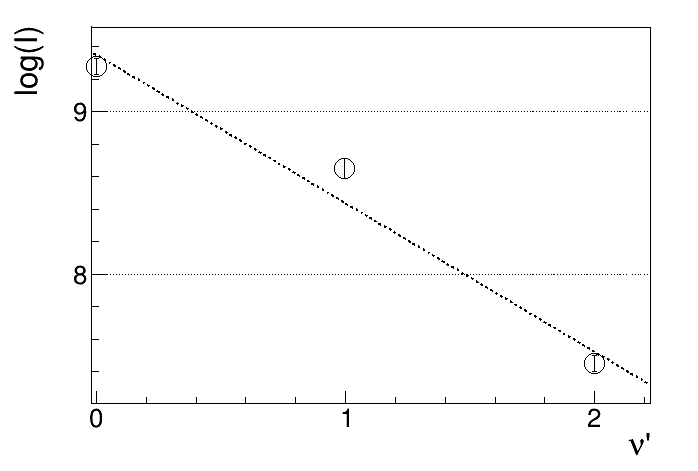
\includegraphics[width=0.48\textwidth]{Images/Spectroscopy/boltzman_f5t16v_2.png}
  }
  \hfill
  \subfloat[vibrational temperature of \ce{N2}]{
    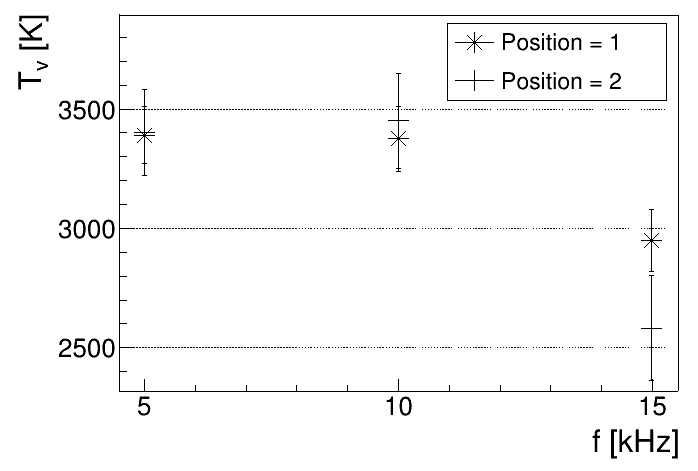
\includegraphics[width=0.48\textwidth]{Images/Spectroscopy/TvN2_2.png}
  }
  \caption{Example of boltzmann graph for estimation of vibrational temperature (a), for discharge with $f = \SI{5}{\kilo\hertz}$, $\Delta t = \SI{16}{\micro\second}$, lens in position 1 and ibrational temperatures of \ce{N2} molecule (b), for different pulse paramters settings, emission measured from position 1 and 2.}
  \label{fig:TvN2}
\end{figure}

\begin{comment}
La determinazione delle specie reattive prodotte dal plasma a pressione atmosferica può essere effettuata tramite misure spettrometriche della sorgente in funzione su un bersaglio.
Gli effetti del trattamento al plasma si pensano dovuti alla presenza di ROS e RNS, quindi vengono raccolte misure nel range di lunghezze d'onda utili ad osservare le emissioni di molecole di \ce{OH} (\SI{305.00}-\SI{313.00}{\nano\meter}), \ce{N_{2}} (\SI{280.00}-\SI{500.00}{\nano\meter}) e \ce{NO} (\SI{220.0}-\SI{290.0}{\nano\meter}) (vedi articoli).

I prototipi di sorgente sviluppati permettono di variare il range dei parametri di funzionamento, in modo da modulare l'intensità del trattamento. Per verificare come cambia lo spettro in base alle diverse modalità di funzionamento, si osservano la variazione nell'intensità delle emissioni al cambiare di frequenza e tempo di apertura del circuito.

Si vuole osservare l'intensità relativa delle righe al variare del gas in ingresso, quindi la sorgente viene azionata con diverse miscele di gas. La misura standard viene effettuata con flusso di \ce{He}, nella solita modalità di funzionamento della sorgente. Vengono poi predisposte due ulteriori modalità di misura dove il gas viene fatto gorgogliare in una soluzione di acqua o di ammoniaca prima dell'inserimento all'uscita della sorgente, per arricchire i prodotti delle reazioni di ioni contenenti, rispettivamente, ossigeno o azoto.

A partire dalla forma delle righe di alcune specie molecolari, è inoltre possibile stimare la temperatura rotazionale alla quale avviene l'emissione misurata. Le emissioni dovute alla molecola \ce{OH} o \ce{N_2} sono varie righe dalle intensità variabili a seconda della temperatura delle molecole, misurando l'intensità relativa dei picchi si può ricavare la temperatura rotazionale delle molecole.

\section{Setup di acquisizione}

Per la sorgente vengono utilizzati sia il prototipo precedente, \textbf{prototipo 1} , sia il prototipo svilupato durante questo lavoro, \textbf{prototipo 2}.

Vengono inoltre provate tre diverse modalità di funzionamento della sorgente, variando frequenza e tempo di chiusura del circuito, mostrate in Tabella \ref{tab:setsorgente}.
Il flusso del gas di elio viene mantenuto pari a \SI{2}{\liter/\minute}.

\begin{table}
 \centering
 \begin{tabular}{cc}
 \toprule
 $f$ [\si{\kilo\hertz}]  &$\Delta t$ [\si{\micro\second}]\\
 \midrule
 5  &15\\
 10 &10\\
 15 &10\\
 \bottomrule
 \end{tabular}
 \caption{Parametri di funzionamento utilizzati per le diverse misure.}
 \label{tab:setsorgente}
\end{table}



\section{Presentazione ed analisi misure}
Per entrambe le sorgenti, l'analisi prevede il riconoscimento delle emissioni misurate, il confronto delle intensità variando distanza e parametri di funzionamento della sorgente, il confronto delle intensità variando il gas immesso, la stima delle temperature rotazionali delle molecole \ce{OH} e \ce{N_2}.

\subsection{Riconoscimento righe}
L'output dello spettrometro viene letto tramite routine IDL ed il riconoscimento dei picchi viene effettuato tramite la classe TSpectrum presente nelle librerie ROOT. Ogni misura viene confrontata con uno spettro di background preso con lo stesso tempo di acquisizione e sorgente spenta, riuscendo così ad escludere i picchi dovuti al fondo.
In figura \ref{fig:spettrotot} si vedono le principali righe estrapolate dalle acquisizioni, in particolare si vedono le righe relative ad \ce{NO}, \ce{OH}, \ce{H_{2}} e \ce{N_{2}}, tabulate in Tabella \ref{tab:spettrotot} .

\begin{figure}
\centering
\includegraphics[width=0.99\textwidth]{Immagini/spettrotot_unico_label_def.png}
\caption{Spettro acquisito con condizioni di misura standard ($f = \SI{5}{\kilo\hertz}$ e $\Delta t = \SI{16}{\micro\second}$), obiettivo puntato vicino l'uscita del gas dalla sorgente.}
\label{fig:app}
\end{figure}


L'acquisizione migliore, nella quale vengono riconosciuti più picchi, è quella mostrata in Figura \ref{fig:spettrotot}, corrispondente alla posizione 1 e condizioni standard di misura, $f = \SI{5}{\kilo\hertz}$.

\paragraph{}
Per verificare gli effetti di una diversa frequenza  nel funzionamento della sorgente vengono confrontate le intensità relative alle righe di \ce{OH} e \ce{N_2}, sommando i conteggi per le varie porzioni di spettro. Non vengono prese in considerazione le righe del gruppo relativo all'\ce{NO} in quanto troppo deboli. In Tabella \ref{tab:irel_1} i risultati, dove vengono confrontate i conteggi alle varie frequenze rispetto i conteggi ottenuti nelle condizioni standard di lavoro, $f = \SI{5}{\kilo\hertz}$. Si nota un calo evidente nei conteggi, crescente con l'aumentare della frequenza di lavoro.

Allo stesso modo viene variata la posizione dell'obbiettivo, dalla posizione 1, puntato all'uscita della sorgente, alla posizione 2, puntato all'uscita del bersaglio. I risultati sempre in Tabella \ref{tab:irel_1}, dove vengono presentati i conteggi nella posizione 2 rispetto i conteggi nella posizione 1. Viene trovato un effetto diverso sulle diverse specie, le emissioni di \ce{OH} diminuiscono molto, mentre quelle relative l'\ce{N_2} diminuiscono in maniera inferiore.

\begin{table}
 \centering
 \begin{tabular}{lcc}
 \toprule
                            &\ce{OH}  &\ce{N_2}\\
 \midrule
 f = \SI{5}{\kilo\hertz}    &1.00     &1.00\\
 f = \SI{10}{\kilo\hertz}    &0.95    &0.81\\
 f = \SI{15}{\kilo\hertz}    &0.62    &0.63\\
 \midrule
 posizione 1                &1.00        &1.00\\
 posizione 2                &0.10     &0.82\\
 \bottomrule
 \end{tabular}
 \caption{Intensità relative delle porzioni interessanti di spettro, al variare di frequenza e posizione, per il prototipo 1.}
 \label{tab:irel_1}
\end{table}


\subsection{\ce{He} + \ce{H_2O} e \ce{He} + \ce{NH_3}}
Vengono misurati gli spettri di emissione in condizioni di lavoro standard, $f = \SI{5}{\kilo\hertz}$, posizione 1, trattando il flusso di elio prima di inserirlo nella sorgente.
Per il prototipo 1, l'arricchimento di specie reattive dell'ossigeno o dell'azoto avviene facendo gorgogliare l'elio in una soluzione di acqua o ammoniaca, mantenendo un flusso in uscita dalla bombola sempre di \SI{2}{\liter/\minute}.
Le misure così acquisite presentano un'intensità molto minore per tutte le righe dello spettro e non vi sono variazioni rilevanti per le lunghezze d'onda interessate, cioè le emissioni relative ad \ce{OH} per la soluzione di acqua e relative ad \ce{N_2} per la soluzione di ammoniaca.

\subsection{Stima temperatura}
Lo spettro di emissione della molecola \ce{OH} è della forma presentata in Equazione \ref{eq:fitOH} (vedi articolo):
\begin{equation}
\centering
\begin{split}
&I_i (T) = I_{0,i} \exp{-\frac{E_n (T-T_0)}{T_0 T}} \\
&S_i(\lambda,T) = \frac{I_i(T)}{\sigma \sqrt{2\pi}} \exp{\frac{(\lambda - \lambda_i)^2}{2\sigma^2}}\\
&S(\lambda,T) = \sum_i S_i(\lambda,T)
\end{split}
\label{eq:fitOH}
\end{equation}

dove $I_i$ è l'intensità ad una determinata energia $E_n$ e $I_{0,i}$ è l'intensità misurata ad una temperatura di riferimento $T_0$. Le $S_i$ sono la convoluzione di $I_i$ con una distribuzione gaussiana nelle $\lambda$ e lo spettro finale $S$ sarà la somma degli spettri relativi la singola transizione.
Simulando diversi spettri nelle varie temperature, sarà possibile stimare la temperatura rotazionale degli ioni presenti nel gas.

La procedura consiste nel simulare diversi spettri $S(\lambda,T)$ come presentati in \ref{eq:fitOH}, calcolare gli scarti quadratici medi rispetto le misure e ricavare la temperatura dalla simulazione migliore. Tipicamente sono stati simulati spettri con $200$ temperature diverse, su un range di temperature possibili variabili, a seconda della misura considerata.
L'errore sulla stima della temperatura viene calcolato come media della differenza tra la temperatura minima che avesse uno scarto quadratico medio fino al $5\%$ superiore rispetto al minimo e la differenza della temperatura massima con le stesse condizioni.

In figura \ref{fig:fitT} sono presentati due esempi di fit delle emissioni interessate. In \ref{tab:Trot} vengono presentate le diverse temperature ottenute, compatibili tra loro.

\begin{figure}
 \centering
 \subfloat[][\ce{OH}]
  {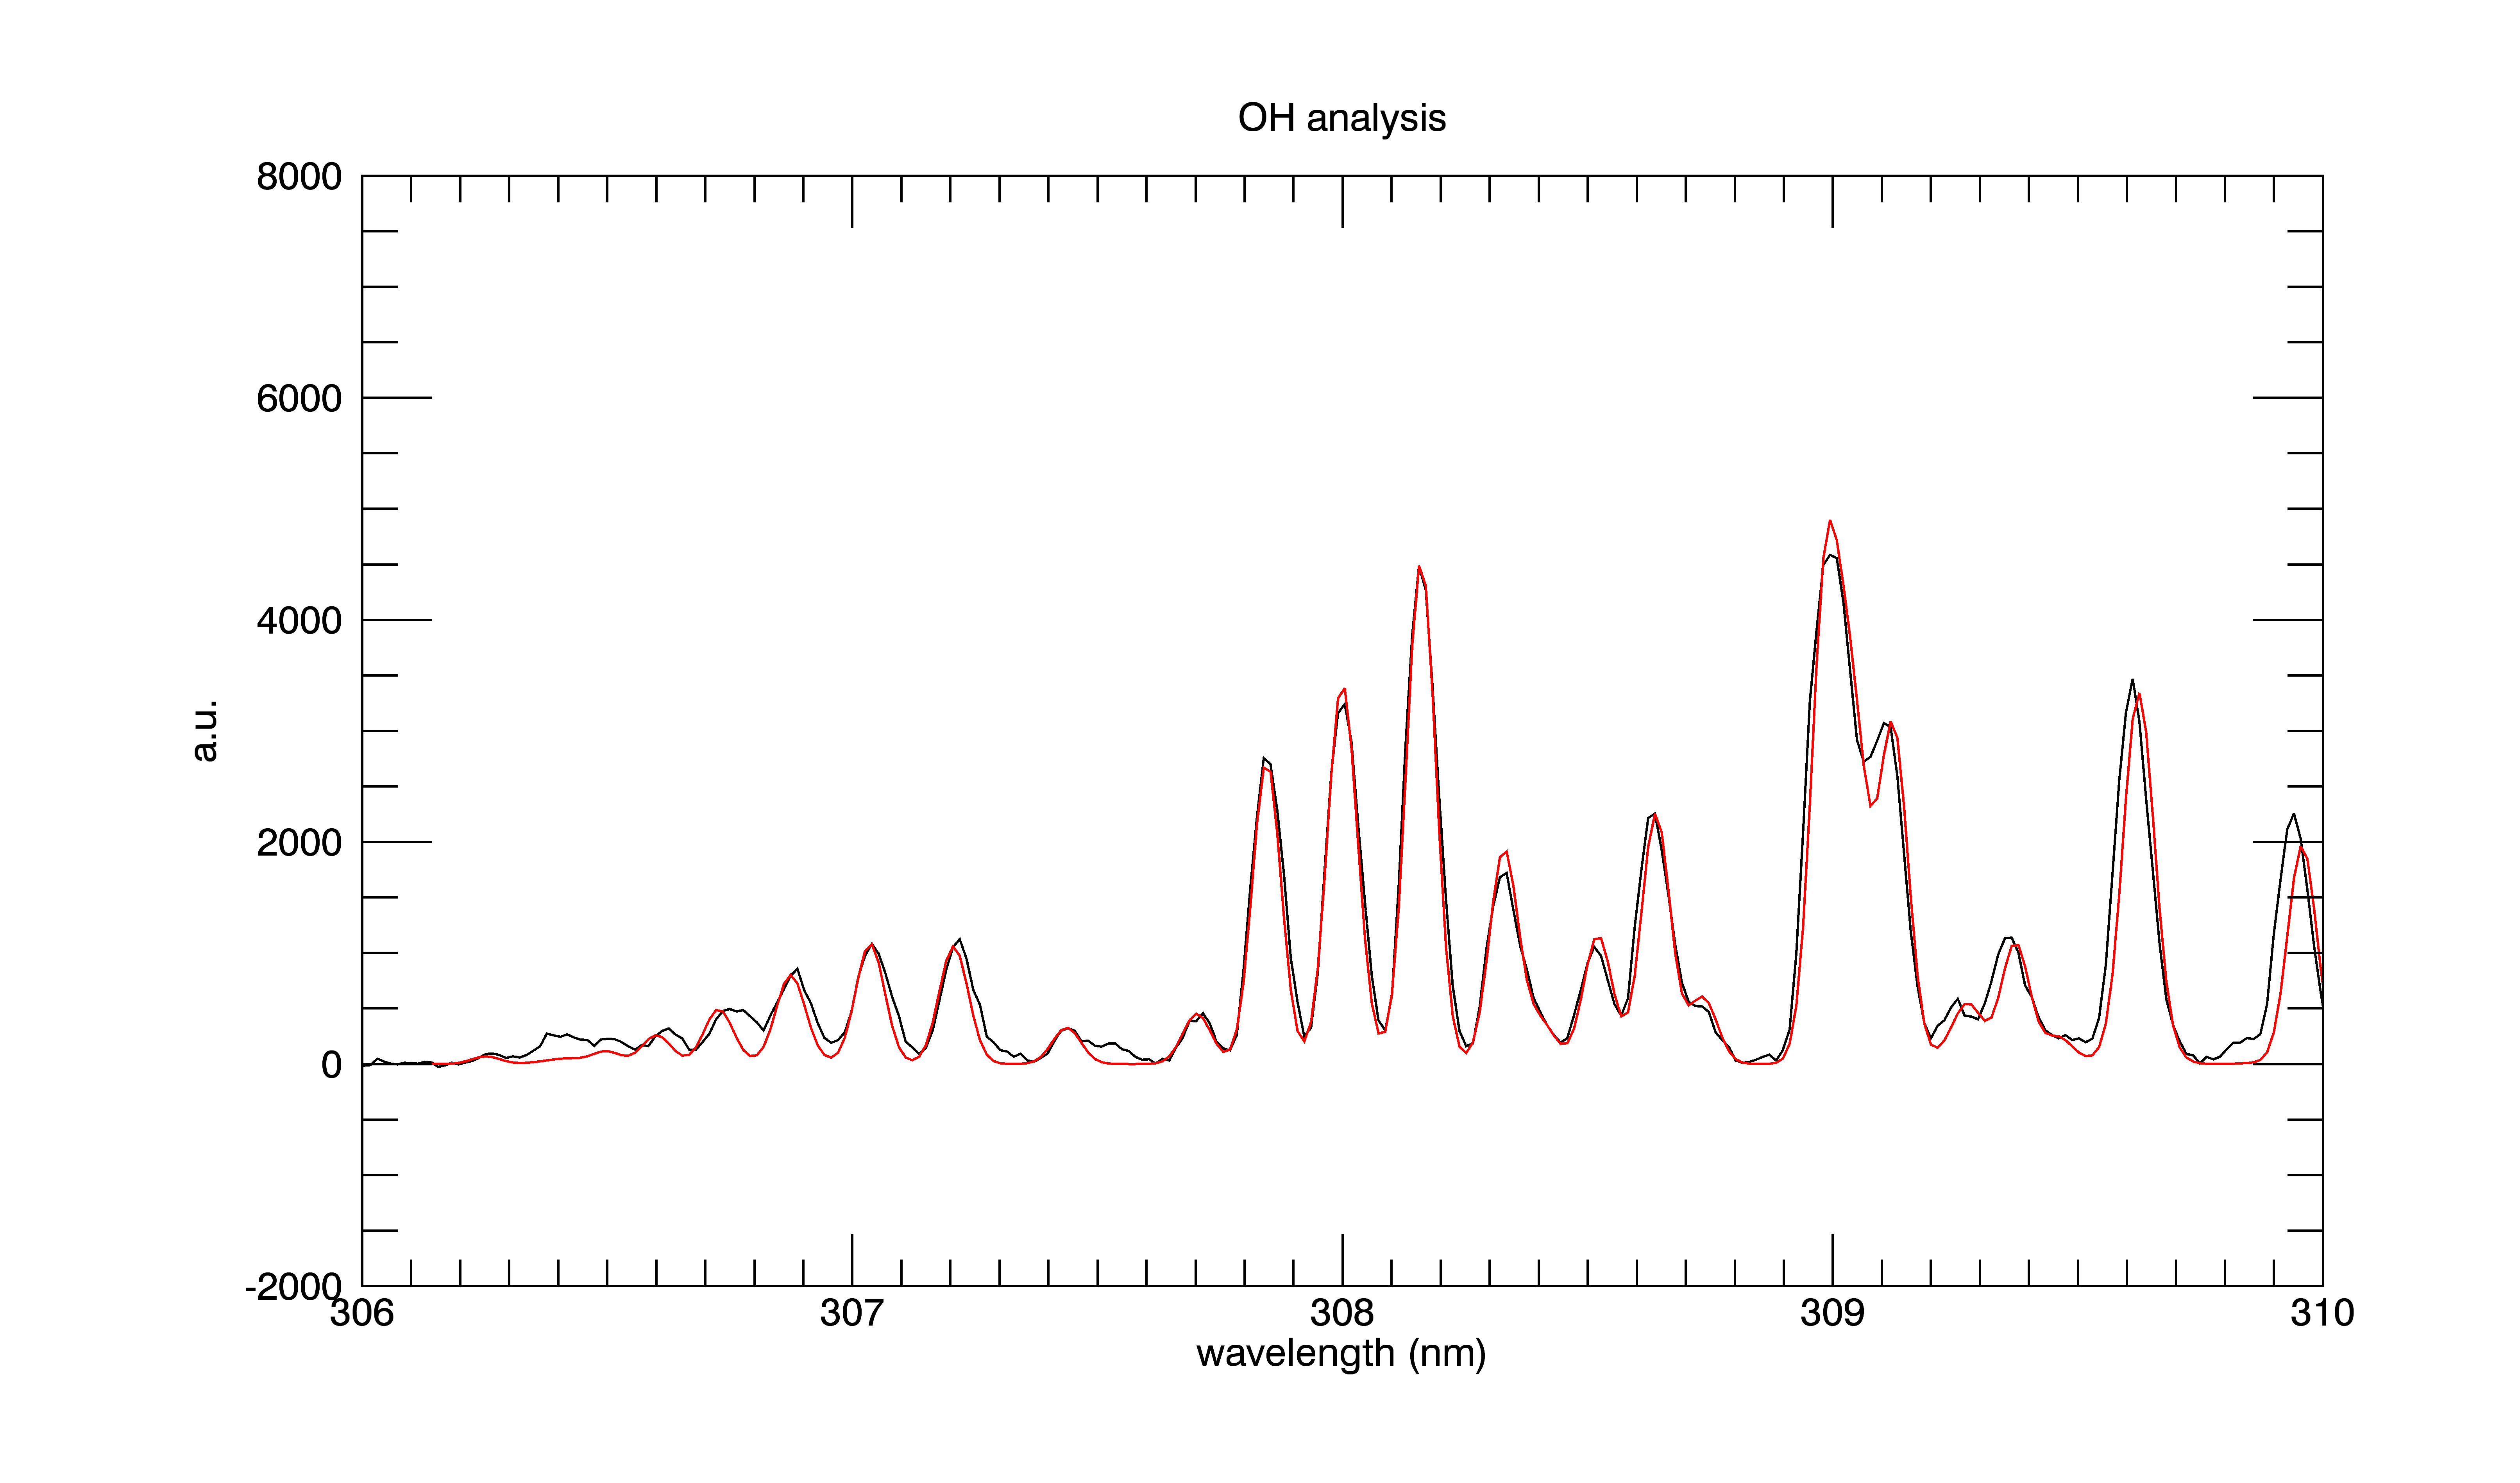
\includegraphics[width=.8\textwidth]{Immagini/OHFit_f5t16elio.png}}
 \\
 \subfloat[][\ce{N_2}]
  {\includegraphics[width=.75\textwidth]{Immagini/N2rotFit_elio.png}}
 \caption{Fit delle emissioni con spettri simulati, misure prese con il prototipo 1, in condizioni standard, posizione 1.}
 \label{fig:fitT}
\end{figure}

\begin{table}
 \centering
 \begin{tabular}{cc}
 \toprule
            &T [\si{\kelvin}]\\
 \midrule
  \ce{OH}   &$336 \pm 30$\\
  \ce{N_2}  &$322 \pm 41$\\
 \bottomrule
 \end{tabular}
 \caption{Stima delle temperature di rotazione delle molecole.}
 \label{tab:Trot}
\end{table}
\end{comment}

\begin{comment}
La misura viene effettuata tramite uno spettrometro IsoPlane dalla lunghezza focale di \SI{320}{\milli\meter}, con tre diversi reticoli: \SI{150}, \SI{1200} e \SI{2400}{g/\milli\meter}, corrispondenti alle risoluzioni di ... .
La risoluzione maggiore viene utilizzata per acquisire le righe \ce{OH} e \ce{N_{2,\text{rot}}}, mentre per acquisire lo spettro totale vengono utilizzati i reticoli a piccola e media risoluzione.

Lo spettrometro è accoppiato ad una telecamera PIXIS di $2048 \times $ ... pixels quadrati dal lato di ... \si{\micro\meter}, con un massimo di \SI{65000} conteggi per il singolo canale.
La luce viene raccolta da una lente in quarzo di focale ... e diametro ... , portata da una fibra ottica dallo spessore di ... e lunghezza di ... e collegata all'entrata dello spettrometro.

Per l'acquisizione viene posizionata la sorgente in funzione a distanza di \SI{1}{\centi\metre} dal bersaglio in metallo (collegato a terra) con l'ottica focalizzata sul flusso di gas, come in foto \ref{fig:app}. Vengono distinte due posizioni dell'ottica:
\begin{itemize}
 \item posizione 1 = obiettivo sull'uscita della sorgente
 \item posizione 2 = obiettivo sul punto di impatto del plasma sulla sorgente, ad \SI{1}{\centi\meter} dall'uscita della sorgente
\end{itemize}
.

\begin{table}
\centering
 \begin{tabular}{ccc}
  \toprule
                            &$\lambda$ \text{[}\si{\nano\meter}\text{]} &\text{I [arb.u.]}\\
  \midrule
  \multirow{4}*{\ce{NO}}    &\num{236.31(24)}  &27\\
                            &\num{237.00(15)}  &26\\
                            &\num{247.02(5)}  &28\\
                            &\num{247.86(12)}  &27\\
  \midrule
  \multirow{2}*{\ce{OH}}    &\num{308.3(1)}  &106\\
                            &\num{309.1(1)}  &113\\
  \midrule
  \multirow{5}*{\ce{N_2}}   &\num{316.03(1)}  &381\\
                            &\num{337.11(1)}  &1000\\
                            &\num{357.77(1)}  &722\\
                            &\num{367.22(20)}  &58\\
                            &\num{371.12(4)}  &172\\
                            &\num{375.66(2)}  &232\\
                            &\num{380.64(2)}  &423\\
  \midrule
  \multirow{2}*{\ce{N_2^+}} &\num{391.50(2)}  &355\\
                            &\num{427.45(2)}  &180\\
  \midrule
  \ce{H_{\alpha}}           &\num{655.96(4)}  &113\\
  \midrule
  \multirow{2}*{\ce{He}}    &\num{586.94(5)}  &122\\
                            &\num{705.56(1)}  &649\\
  \midrule
  \ce{O}                    &\num{776.39(1)}  &393\\
  \bottomrule
 \end{tabular}
 \caption{Picchi rilevanti nello spettro di emissione del prototipo 1, condizioni di misura standard, posizione 1.}
 \label{tab:spettrotot}
\end{table}


Per ogni misura viene stabilito un tempo di acquisizione idoneo ad avere un numero ottimale di eventi, evitando la saturazione dei singoli canali. Una volta stabilito il tempo viene eseguita una misura di fondo, a sorgente spenta, e successivamente viene avviata la misura con sorgente attiva.
\end{comment}
